%███████████████████████████████████████████████████████████████████
%███████████████████████████████████████████████████████████████████
%███████████████████████████████████████████████████████████████████
%███████████████████████████████████████████████████████████████████
%███████████████████████████████████████████████████████████████████
%███████████████████████████████████████████████████████████████████
\chapter{Conclusion}\label{ch: Conclusion}
% \chapter{Outro}

This handbook of special relativity has gone through a lot.
However, there is still plenty I have yet to distill, and I will hopefully include more sections when I get the time.
For now, I hope this handbook was useful to you.
If you are still looking for more in the meantime, there are plenty of external resources in chapter (\ref{ch: Resources}) to expand your knowledge and give you some different perspectives and mental practice.

I will leave you with a final note on gravity and its role in relativity.

% some things to keep in mind when working with all the concepts, then

% %███████████████████████████████████████████████████████████████████
% %███████████████████████████████████████████████████████████████████
% \section{Things to Remember}\label{sect: Things to Remember}

% *** maybe just remove for now

% *** when using special relativity, it is important to remember the basics of setting up the mathematical model of you inertial reference frame, and carefully choosing the time $\TtPRM=0$ and $\Tt=0$ when the two coordinate system's axis of each frame overlap.


% * there is no such thing as a truly rigid body, i.e. a box or a stick are not truly rigid, if one part starts to move at a different rate to the rest the signal/force passes less than or equal to the speed of light to the rest of the parts deforming it, with the gap between atoms changing to do so. this has to be taken into account.
% * There is a thought experiment by Einstein of light in a box, being emitted from one side of the box to the other, it was used to argue to get the equation for the momentum of light, its is a simple thought experiment, but i did not include it as it relied on a rigid box, and I did not want to rely on assumption that it applied none rigid bodies too


% *** Questions you may have
% *** General confusions

%███████████████████████████████████████████████████████████████████
%███████████████████████████████████████████████████████████████████
\section{A Note on Gravity}\label{sect: A Note on Gravity}

For a reference frame to be inertial there has to be zero acceleration, but the gravity of the earth and other masses accelerates objects towards them.
Out in space, we still have this acceleration even though it may be weak, so special relativity can actually only be used as an approximation when modeling a system.
Where gravity is stronger or time scales are much longer and these approximations are not good enough, we require an even more complex view of the world and the next level of frame transformations, between two non-inertial frames of reference.
This is where general relativity comes in.
It is used to explain the redshift of light from stars and also the bending of light around massive stars.
It also explains the difference in the flow of time at different strengths of gravity; this gravitational time dilation has to be taken into account by the satellites used by GPS systems.
But there are downsides to general relativity, such as its incompatibility with quantum mechanics, its failure to explain why galaxies rotate much faster than they should based on the visible matter, and its failure to explain why the expansion of the universe is accelerating.
It requires inventing new invisible entities to explain these, called dark matter and dark energy (which are vague concepts, as they are whatever new particles or physics are invented that happen to describe some of the discrepancy in the gravity well enough).
However, these concepts still fail in many cases.
There is also a competitor theory called MOND (Modified Newtonian Dynamics).
While it clears up some discrepancies, it fails in many other instances.

So the correct theory and full description of gravity is still to be decided.

But if you want to start learning more about gravity, the thought experiment that started general relativity is undeniably a perfect starting point.

%███████████████████████████████████████████████████████████████████
\subsection{Elevator Thought Experiment and the Equivalence Principle}
\label{subsect: Elevator Thought Experiment and the Equivalence Principle}

If you were in an elevator in free fall, you would feel weightless, as you would also be free-falling at the same speed, and feel no force from the floor of the elevator into your feet, just like the springs feel no force in the inertial frame in the first diagram of Figure (\ref{fig: spring boxes}).
You would also feel the same weightlessness if you were in an elevator out in deep space, away from any masses.
Even though someone at rest on earth would see you accelerating towards the ground in the free-falling elevator, you would not be able to tell the difference between these two situations from inside the windowless elevators, i.e., the reference frames of both elevators are equivalent.
The free-falling elevator feels as though it is at rest or in an inertial frame of reference.

Now, what about an elevator at rest on earth? If a ball is dropped from rest, as shown in figure (\ref{fig: mass-earth}), it has an acceleration of $\Tgravity$ downwards.

\begin{figure}[htbp]
        \centering
        \tikzsetnextfilename{Ball_in_elevator_on_earth}
        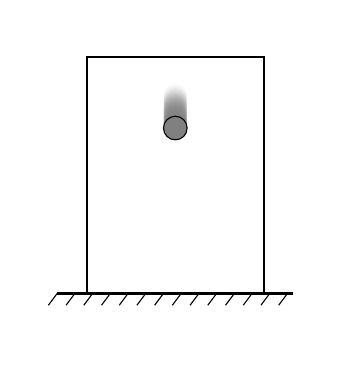
\begin{tikzpicture}[scale=0.75]
            \useasboundingbox (-1, 0.0) rectangle (4, 5.5);

            % Main Elevator
            \draw[thick] (0,1) rectangle (3,5);

            % Ground with diagonal dashes
            \draw[thick] (-0.5, 1) -- (3.5, 1);
            \foreach \x in {-0.5, -0.2, ..., 3.5} {
                \draw (\x, 1) -- (\x-0.15, 0.8);
            }

            % Fading trail of masses above the main one (downward motion blur)
            \foreach \i in {1,...,15} {
                \pgfmathsetmacro{\opacity}{0.5 * (1 - \i/15)}
                \draw[fill=gray, draw=none, opacity=\opacity] (1.5, 3.8 + \i*0.04) circle (0.2);
            }

            % Main Mass inside main elevator
            \draw[fill=gray] (1.5, 3.8) circle (0.2);
        \end{tikzpicture}
        \caption{An elevator at rest, in earth's non-inertial rest frame, showing a ball accelerating towards the earth due to gravity.}
        \label{fig: mass-earth}
\end{figure}

Now, what if we apply the same acceleration to the elevator in deep space?
In an inertial frame outside the elevator we would see the elevator accelerate towards the ball, as shown in figure (\ref{fig: mass-space-out}).
But inside the elevator, in its non-inertial frame, we would see the ball accelerate towards the elevator floor at the same acceleration as the elevator at rest on earth, as shown in figure (\ref{fig: mass-space-out}).
You would also feel the same weight on your feet.
Again, the frames of both of these elevators are equivalent.

\begin{figure}[htbp]
    \centering
    \begin{subfigure}[b]{0.45\textwidth}
        \centering
        \tikzsetnextfilename{Ball_in_accelerating_elevator_in_inertial_frame}
        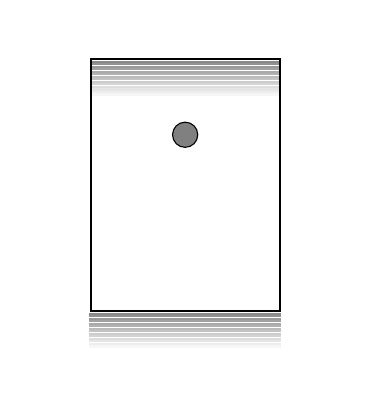
\begin{tikzpicture}[scale=0.8]
            \useasboundingbox (-1, 0.0) rectangle (4, 5.5);

            % Fading horizontal lines for the top and bottom edges (upward motion blur)
            \foreach \i in {1,...,15} {
                \pgfmathsetmacro{\opacity}{0.5 * (1 - \i/15)}
                % Bottom edge trail
                \draw[thick, opacity=\opacity] (-0.02, 1 - \i*0.04) -- (3.02, 1 - \i*0.04);
                % Top edge trail
                \draw[thick, opacity=\opacity] (0, 5 - \i*0.04) -- (3, 5 - \i*0.04);
            }

            % Main Elevator
            \draw[thick] (0,1) rectangle (3,5);

            % Mass inside main elevator
            \draw[fill=gray] (1.5, 3.8) circle (0.2);
        \end{tikzpicture}
        \caption{Accelerating elevator in space, inertial frame}
        \label{fig: mass-space-out}
    \end{subfigure}
    \hfill
    \begin{subfigure}[b]{0.45\textwidth}
        \centering
        \tikzsetnextfilename{Ball_in_accelerating_elevator_in_elevators_frame}
        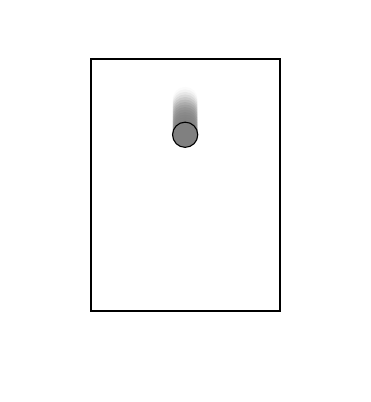
\begin{tikzpicture}[scale=0.8]
            \useasboundingbox (-1, 0.0) rectangle (4, 5.5);

            % Main Elevator
            \draw[thick] (0,1) rectangle (3,5);

            % Fading trail of masses above the main one (downward motion blur)
            % draw=none prevents the black outlines from compounding
            \foreach \i in {1,...,15} {
                \pgfmathsetmacro{\opacity}{0.5 * (1 - \i/15)}
                \draw[fill=gray, draw=none, opacity=\opacity] (1.5, 3.8 + \i*0.04) circle (0.2);
            }

            % Main Mass inside main elevator
            \draw[fill=gray] (1.5, 3.8) circle (0.2);
        \end{tikzpicture}
        \caption{Accelerating elevator in space, elevator's frame}
        \label{fig: mass-space-in}
    \end{subfigure}
    \caption{A ball in an accelerating elevator in deep space, with an inertial frame (left) showing a stationary ball with the elevator accelerating upwards, and also the elevators non-inertial rest frame (right), showing the stationary elevator with the ball accelerating downwards.}
    \label{fig: elevator-mass}
\end{figure}



So the mass released from rest behaves identically whether the elevator is accelerating upwards in deep space at $\Tgravity$ or sitting stationary on the surface of the earth experiencing a gravitational pull of $\Tgravity$.

Formally, the gravitational equivalence principle states that there is no local physical experiment you can perform to distinguish between being in a uniform gravitational field and being in a uniformly accelerating reference frame.

Let us now see how this equivalence allows us to deduce that gravity bends the path of light.

If we are in an inertial reference frame outside the elevator in deep space, and shine a light horizontally through a hole in the elevator, it will travel in a straight line across the elevator in this inertial frame.
But the elevator is accelerating, and as the light moves across, the elevator rises up more and more quickly, and the light hits the other side of the elevator at a lower point, as shown in figure (\ref{fig: light-straight}).
From the non inertial frame, inside the elevator, we would see the path of light bend downwards and hit the wall at the lower point, as shown in figure (\ref{fig: light-straight}).

\begin{figure}[htbp]
    \centering
    \begin{subfigure}[b]{0.45\textwidth}
        \centering
        \tikzsetnextfilename{Light_in_accelerating_elevator_in_inertial_frame}
        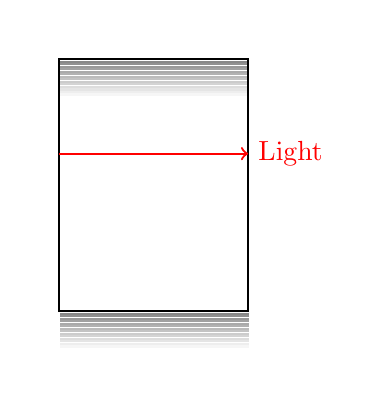
\begin{tikzpicture}[scale=0.8]
            % Bounding box adjusted to remove the old y=-1 space
            \useasboundingbox (-0.5, 0) rectangle (4.5, 5.5);

            % Fading horizontal lines for the top and bottom edges (upward motion blur)
            \foreach \i in {1,...,15} {
                \pgfmathsetmacro{\opacity}{0.5 * (1 - \i/15)}
                % Bottom edge trail
                \draw[thick, opacity=\opacity] (0.02, 1 - \i*0.04) -- (3.02, 1 - \i*0.04);
                % Top edge trail
                \draw[thick, opacity=\opacity] (0, 5 - \i*0.04) -- (3, 5 - \i*0.04);
            }

            % Current elevator position
            \draw[thick] (0,1) rectangle (3,5);

            % Light ray
            \draw[thick, red, ->] (0, 3.5) -- (3, 3.5) node[right] {Light};
        \end{tikzpicture}
        \caption{Accelerating elevator in space, inertial frame}
        \label{fig: light-straight}
    \end{subfigure}
    \hfill
    \begin{subfigure}[b]{0.45\textwidth}
        \centering
        \tikzsetnextfilename{Light_in_accelerating_elevator_in_elevators_frame}
        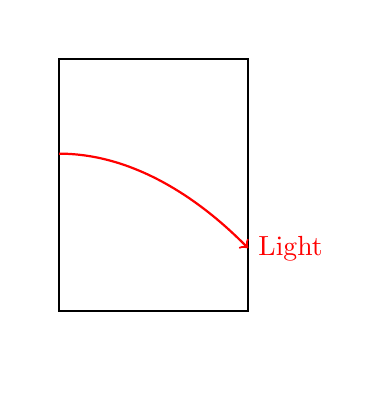
\begin{tikzpicture}[scale=0.8]
            % Bounding box adjusted to perfectly match the left figure
            \useasboundingbox (-0.5, 0) rectangle (4.5, 5.5);

            % Elevator (already matches height of current elevator in subfigure a)
            \draw[thick] (0,1) rectangle (3,5);

            % Light ray (curved, shifted relative to the new elevator height)
            \draw[thick, red, ->] (0, 3.5) parabola (3, 2) node[right] {Light};
        \end{tikzpicture}
        \caption{Accelerating elevator in space, elevator's rest frame}
        \label{fig: light-curved}
    \end{subfigure}
    \caption{An accelerating elevator in deep space, with light traveling across it, with an inertial frame (left) showing a straight light path across the elevator while the elevator accelerates upwards, and also the elevator's non-inertial rest frame (right), showing the stationary elevator with the light's path bent downward.}
    \label{fig: light-frames}
\end{figure}

The light's path is bent in the non inertial frame, but from the equivalence principle, the frame inside an elevator at rest on earth is equivalent, since it experiences the same acceleration due to gravity.
So we would then expect to find that gravity does, in fact, bend the light by the same amount, shown in figure (\ref{fig: equiv-earth}).
This has been experimentally verified: light does indeed bend around heavy masses such as stars, black holes, and to a lesser extent, planets.

\begin{figure}[htbp]
    \centering
    \tikzsetnextfilename{Light_in_elevator_at_rest_on_earth}
    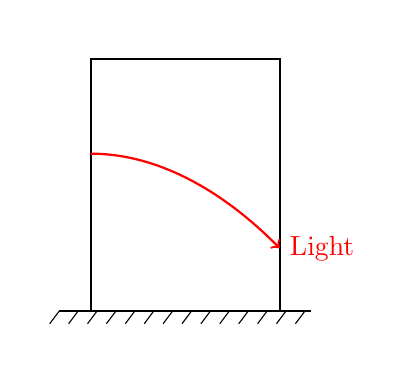
\begin{tikzpicture}[scale=0.8]
        \useasboundingbox (-1, -0.5) rectangle (4.5, 4.5);
        % Elevator
        \draw[thick] (0,0) rectangle (3,4);
        % Ground with diagonal dashes
        \draw[thick] (-0.5, 0) -- (3.5, 0);
        \foreach \x in {-0.5, -0.2, ..., 3.5} {
            \draw (\x, 0) -- (\x-0.15, -0.2);
        }
        % Light ray (curved)
        \draw[thick, red, ->] (0, 2.5) parabola (3, 1) node[right] {Light};
    \end{tikzpicture}
    \caption{An Elevator at rest on earth, in the earth's non-inertial frame, with light being bent towards the ground, as it is equivalent to the scenario with the accelerating elevator in deep space.}
    \label{fig: equiv-earth}
\end{figure}

In the real world, the gravitational field in the elevator on earth is not perfectly uniform, but it is a good approximation.
The top of the elevator is further from earth and so gravity is a slightly weaker than at the bottom.
Also, for a spherical mass, the gravitational field spreads out spherically, creating a negligible difference in the gravitational strength in the center of the elevator compared to the walls; this is called a tidal force.
These are negligible effects for our thought experiment, but might be significant when modeling other systems.

In general relativity, the local speed of light is always equal to $\Tc$ according to the observer who is there. But when viewed from a different gravitational strength, it appears to be moving at a different speed.
This effect is tied to gravitational time dilation, which we will give a note about next.

%███████████████████████████████████████████████████████████████████
\subsection{Gravitational Time Dilation}\label{subsect: Gravitational Time Dilation}

We have seen the time dilation equation in special relativity between two reference frames, but gravity also has a time dilation associated with its strength.
The stronger the gravity at a point, the slower time passes relative to an inertial reference frame that doesn't experience any gravitational force.

\begin{equation}
     \TDtg = \TDtinf \sqrt{1 - \frac{\Tvesc^2}{\Tc^2}}
\end{equation}

Where $\Tvesc$ is the minimum velocity an object has to be traveling away from a mass to escape its orbit, and $\TDtg$ is the change in time within a gravitational well compared to the change in time at an infinite distance away $\TDtinf$.
This is the same as the time dilation in special relativity as seen in equation \eqref{eq: time dilation} if we were to use $\Tv=\Tvesc$.
The escape velocity is also the same velocity (but in the opposite direction) that a particle would have if it started at rest an infinite distance away and reached the current position in a stationary mass's gravitational field.
There is an interpretation of general relativity called the "river model" \cite{rivermodel}, which suggests that gravity and its effects are due to space itself falling inwards at this velocity at each point.
It also extended this to rotating masses.
This model is an interpretation that can be useful for learning general relativity, but it is a niche interpretation.
So, you can keep an open mind about it and remain skeptical about whether the interpretation is worthwhile.

This concludes The Handbook of Special Relativity, but please check out the other resources on this topic that I have provided in the next bit.


% *** what about light coming out of a masses gravity field, how does its non local speed change from a point on the event horizon to infinity, for someone at infinity, also is it different depending on its direction its moving


%- [ ] this was meant as an introduction to physical concepts and mathematical tools
%- [ ] propose areas of expansion for this topic/ future research